\section{React Native}
\label{reactnative}

\subsection{Was ist React Native?}
React Native ist ein JavaScript-Framework, welches dafür verwendet wird, Cross-Platform-Apps für
die Betriebssysteme Android, iOS, Windows und MacOS zu entwickeln. Außerdem ist der Zugriff auf die
native Plattform-API möglich.

\subsubsection{Wie viel React steckt wirklich in React Native?}
Wie der Name schon vermuten lässt baut React Native hauptsächlich auf die JavaScript-Bibliothek
React auf. Sie hilft bei der Erstellung der Benutzeroberfläche, verwaltet den Zustand der
Anwendung und hat noch viele weitere kleine Aufgaben. React an sich ist noch eine Bibliothek,
mit -- absichtlich -- wenig "Grundgerüst". Das macht es auch für die Open-Source-Gemeinschaft
einfacher zusammen gute Lösungen zu entwickeln und so werden die wenigen wichtigen Aufgaben von
React dafür perfekt ausgeführt.
Detaillierte Informationen zu State, Render-Funktionen, Komponenten und JSX finden Sie im Kapitel
\nameref{reactjs}.

\subsubsection{Geschichte}
Die ersten Versionen der Facebook-App für Smartphones war eine Hybrid-App, also eine Webseite,
welche einfach in einer nativen App eingebunden wird \cite{reactNativeHistory}. Die Leistung der
Handy-App war für das Niveau des Social-Media-Giganten eindeutig zu schlecht, die App musste neu
geschrieben werden in Objective-C, womit Facebook sich eine 2,5-fach schnellere Anwendung erwartete
\cite{facebookNewIosApp}.

Nachdem React veröffentlicht worden war, versuchten die Entwickler bei Facebook einen effizienten
Weg zu finden, die neue Technologie zu nutzen um native Anwendungen, genauer eigentlich
Cross-Platform Anwendungen, zu schreiben.

2015 wurde die erste stabile Version von React Native veröffentlicht. Seit Anfang an verwendet
Facebook intern in ihren erfolgreichsten Apps React Native als Basistechnologie. Die Firma Microsoft
stellt selbst Bibliotheken zur Verfügung, um React Native Anwendungen auch für die Universal Windows
Platform (UWP) und MacOS zu entwickeln.

\newpage

\subsubsection{Wer benutzt React Native?}
Laut der eigenen Webseite von React Native benutzen einige der größten Firmen der Welt React Native
als Cross-Platform-Framework für ihre Android- und iOS-Apps.

\begin{table}[H]
\centering
\begin{tabular}{|l|l|c|c|l|}
  \hline
  \textbf{Unternehmen} & \textbf{App} & \textbf{Android} & \multicolumn{1}{l|}{\textbf{iOS}} \\ \hline\hline
  \multirow{5}{*}{Facebook} & Facebook             & \multicolumn{2}{c|}{\multirow{5}{*}{\XBox}} \\
                            & Facebook Ads Manager & \multicolumn{2}{c|}{}                       \\
                            & Facebook Analytics   & \multicolumn{2}{c|}{}                       \\
                            & Instagram            & \multicolumn{2}{c|}{}                       \\
                            & Oculus               & \multicolumn{2}{c|}{}                       \\ \hline
  Microsoft                 & Skype                & \multicolumn{2}{c|}{\XBox}                  \\ \hline
  Discord                   & Discord              & \Square          & \XBox                    \\ \hline
  Tesla                     & Tesla                & \multicolumn{2}{c|}{\XBox}                  \\ \hline
  Coinbase                  & Coinbase             & \multicolumn{2}{c|}{\XBox}                  \\ \hline
  Walmart                   & Walmart              & \multicolumn{2}{c|}{\XBox}                  \\ \hline
  Pinterest                 & Pinterest            & \multicolumn{2}{c|}{\XBox}                  \\ \hline
  Uber                      & Uber Eats            & \multicolumn{2}{c|}{\XBox}                  \\ \hline
  Shopify                   & Shopify              & \multicolumn{2}{c|}{\XBox}                  \\ \hline
  Wix.com                   & Wix.com              & \multicolumn{2}{c|}{\XBox}                  \\ \hline
\end{tabular}
\end{table}

\begin{center}
  Berühmte Beispiele für Apps mit React Native \cite{reactNativeShowcase}
\end{center}

Discord ist das einzige Unternehmen in der Liste, welches nur für die Plattform iOS React Native
verwendet. In einem Blog Post erklären sie, dass React Native auf Android ihrer Meinung nach keine
akzeptable Performance in Sachen Reaktionsfähigkeit von Knöpfen liefert \cite{reactNativeDiscord}.
Dieser Post ist aus dem Jahr 2018 und seitdem hat sich React Native stark verbessert. Im selben Jahr
begann nämlich auch die Entwicklung von Fabric, der neuen Render-Engine von React Native, welche
2021 dann schließlich in die offizielle Facebook App übernommen wurde.

\subsubsection{Lizenz}
React Native wird unter der MIT-Lizenz geführt, das heißt dass jeder die Software sowohl für
Open-Source als auch für Closed-Source-Projekte verwenden darf.

\subsection{Erstellung eines React Native Projekts}
Schon bei der Erstellung des Projekts müssen einige Fragen geklärt werden. Als erstes sollte man
sich wohl fragen, mit welcher CLI man das Projekt erstellen möchte.

Mit CLI (für engl. command-line-interface) ist in unserem Kontext eine Sammlung von Befehlen
gemeint, die in der Kommandozeile eines PCs ausgeführt werden können. Beispiele für Kommandozeilen-
Emulatoren:

\begin{itemize}
  \item Windows Powershell
  \item Windows Cmd
  \item MacOS zsh
  \item Git Bash
  \item Gnome Shell
\end{itemize}

\subsubsection{Expo CLI}
\label{expocli}
Die Entwickler von React Native selbst empfehlen allen Anfängern im Gebiet App-Entwicklung die
Verwendung der Expo CLI \cite{expocli}, welche eine vereinfachte Variante einer React Native Anwendung erzeugt.

Als Vorteil zählt auf jeden Fall die Geschwindigkeit, mit der eine neue App auf einem neuen Gerät
getestet werden kann. Dies ist meist innerhalb weniger Minuten möglich.

Ein wichtiger Nachteil ist jedoch, dass man in einem Expo-Projekt eingeschränkten Zugriff auf
Schnittstellen des Betriebssystems hat, es sind im Projekt nicht einmal die Ordner android und ios
vorhanden, um Änderungen vorzunehmen.

\subsubsection{Installation und Erstellung einer Expo App}
Um eine Expo React Native Anwendung erstellen zu können benötigt man als erstes \nameref{nodejs} und
den darin enthaltenen Node Package Manager. In einer Kommandozeile führt man nun folgende Befehle
aus, um die Expo-CLI im globalen Kontext zu installieren und anschließend ein Expo Projekt zu
erstellen. Nach der Auswahl für die Vorlage wir das Projekt erstellt.

\begin{lstlisting}
C:\example> npm install -g expo-cli
added 1549 packages, and audited 1550 packages in 1m

C:\example>expo init expoInitBlank
? Choose a template: - Use arrow-keys. Return to submit.
    ----- Managed workflow -----
>   blank               a minimal app as clean as an empty canvas
    blank (TypeScript)  same as blank but with TypeScript configuration
    tabs (TypeScript)   several example screens and tabs using react-navigation and TypeScript
    ----- Bare workflow -----
    minimal             bare and minimal, just the essentials to get you started
\end{lstlisting}

\subsubsection{Ordnerstruktur}
\begin{figure}[H]
  \begin{center}
    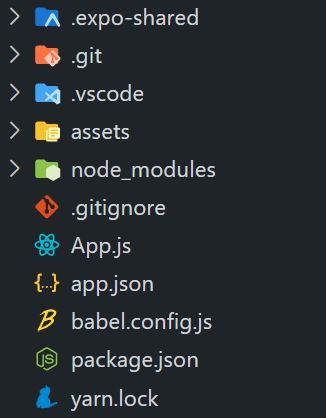
\includegraphics[width=0.5\textwidth]{Theorie/ReactNative/ExpoFolderStructure.JPG}
    \caption{Ordnerstruktur Expo Init Blank}
  \end{center}
\end{figure}

\begin{itemize}
\item Ordner:
\begin{itemize}
\item \textbf{.expo-shared, .git, .vscode}:\\
In den Ordnern .expo-shared, .git und .vscode befinden sich lediglich Konfigurationsdateien für Expo
selbst, die Versionsverwaltungssoftware Git und Visual Studio Code, dem Text-Editor, den wir
durchwegs für die gesamte Diplomarbeit verwendet haben.

\item \textbf{assets}:\\
Der Ordner assets ist für das Abspeichern von statischen Ressourcen, wie Bildern, Icons oder
ähnliches gedacht.

\item \textbf{node\_modules/}:\\
Im Ordner node\_modules werden alle Bibliotheken abgespeichert, die mit Hilfe des Paketmanagers
in das Projekt eingebunden wurden. Expo entschied sich gegen die Verwendung von NPM und verwendet
stattdessen Yarn.
\end{itemize}

\newpage

\item Dateien:

\begin{itemize}
\item \textbf{App.js}\\
Die wichtigste Datei im Projekt ist wohl App.js, sie ist der Einstiegspunkt für die App.

\begin{lstlisting}
import { StyleSheet, Text, View } from 'react-native';

function App() {
  return (
    <View style={styles.container}>
      <Text>Open up App.js to start working on your app!</Text>
    </View>
  );
}

const styles = StyleSheet.create({
  container: {
    flex: 1,
    backgroundColor: '#fff',
    alignItems: 'center',
    justifyContent: 'center',
  },
});

export default App;
\end{lstlisting}

In der ersten Zeile des Programms werden diverse React Native Core Components importiert. Core
Components sind, wörtlich übersetzt, die Kernkomponenten des Frameworks, mit ihnen wird der Großteil
der Benutzeroberfläche aufgebaut. Wie bereits erwähnt, werden die React Native Komponenten beim
Kompilieren in die richtigen Komponenten für das Zielsystem umgewandelt.

\begin{table}[H]
\centering
\begin{tabular}{|l|l|l|l|}
  \hline
  \textbf{Komponente} & \textbf{Android} & \textbf{iOS} & \textbf{HTML} \\ \hline\hline
  View                & ViewGroup        & UIView       & div          \\
  Text                & TextView         & UITextView   & p            \\ \hline
\end{tabular}
\end{table}

\begin{center}
  React Native Core Components und deren Äquivalente im Überblick \cite{reactNativeCoreComponents}
\end{center}

In der nächsten Zeile wird unserer erster React-Component erzeugt, welcher im Grunde nur eine
Funktion ist, die \nameref{jsx}-Code als Rückgabewert liefert.

In Zeile 5 wird zur View ein React Native StyleSheet zugewiesen. Man verwendet nämlich kein
gewöhnliches \nameref{css}, wie in der Webentwicklung, sondern ein relativ ähnlich aufgebautes,
eigenes System zur Gestaltung der App. Ein wichtiger Unterschied ist, dass die Attribut-Namen im
StyleSheet nicht durch Bindestriche getrennt, sondern in der LowerCamelCase-Notation geschrieben
werden \cite{camelCaseNotation}.

Am Ende der Datei wird noch die Komponente als Default exportiert, damit sie von Expo verarbeitet
werden kann \cite{jsModules}.

\item \textbf{app.json, package.json}\\
app.json wird von Expo generiert und mit Metadaten befüllt. In ihr werden Daten abgespeichert,
die nicht in der App selbst eingebaut werden, sondern das Projekt selbst beschreiben, z.B. Name der
App, Versionsnummer, Bildschirmausrichtung und noch viele weiter Optionen.

\begin{figure}[H]
  \begin{center}
    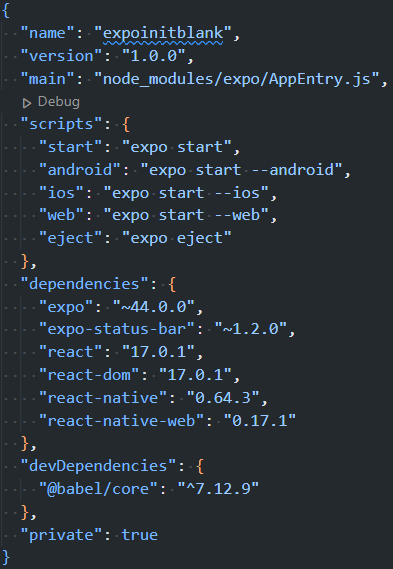
\includegraphics[width=0.5\textwidth]{Theorie/ReactNative/package-json.png}
    \caption{package.json in einem Expo Blank Template}
  \end{center}
\end{figure}

package.json hat einen ähnlichen Zweck, auch darin sind Name, Versionsnummer, aber auch der
Eintrittspunkt in die App abgespeichert. In Scripts werden Kommandozeilenbefehle abgespeichert, die
mit Hilfe des Befehls npm run <script> aufgerufen werden können. Im nächsten Objekt werden die
Namen der Bibliotheken aufgelistet, welche für das Ausführen der App benötigt werden. Bibliotheken,
die nur während der Entwicklung benötigt werden, sind unter devDependencies abzuspeichern (beim
Installieren den Tag -{}-save-dev anhängen).

\item \textbf{package-lock.json, yarn.lock}\\
package-lock.json und yarn.lock haben beide dieselbe Aufgabe, sie sollten jedoch niemals
gleichzeitig im gleichen Projekt existieren. Ersteres gehört nämlich zum Paketmanager NPM, wobei
yarn.lock von Yarn generiert wird. Expo erzeugt ein Blank-Template standardmäßig mit Yarn, man kann
aber auch stattdessen mit dem Tag -{}-npm bei der Projekterstellung NPM einbinden.

\item \textbf{babel.config.js}\\
Babel ist ein sogenannter JavaScript-Transpiler. Er wandelt JavaScript-Features, welche erst in
späteren Versionen des ECMAScript-Standards eingebaut und möglicherweise noch nicht von allen
Systemen unterstützt werden, in JavaScript-Code um, welcher auch von älteren Versionen verstanden
werden kann, um (vgl. ein Compiler wandelt lesbaren Code in Maschinencode um). Außerdem hat er noch
einige andere Funktionen, welche durch Plugins hinzugefügt werden können. In der Konfigurationsdatei
wird nur eine vorgefertigte Liste an Plugins in das Projekt eingebunden, das "babel-preset-expo".

\item \textbf{.gitignore}\\
In die Datei .gitignore fügt man Datei- und Ordnernamen ein, die nicht von der Versionsverwaltung
gesichert werden sollen. Sehr zu empfehlen ist dies beim Ordner node\_modules, da dieser schon
direkt nach der Erstellung 170 Megabytes groß ist und er aus den Dateien package.json und yarn.lock
generiert werden kann.

\end{itemize}
\end{itemize}

\subsubsection{Metro}
\label{metrobundler}
Beim Start der App wird als erstes der Metro Bundler initialisiert. Er besteht aus einem Server,
welcher den geschriebenen Code mittels Babel kompiliert und anschließend an die App schickt. Dadurch
verhindert man, jedes mal die App neu auf das Gerät installieren zu müssen, um eine kleine Änderung
im Text sehen zu können. Beim Einbinden von neuen JavaScript-Bibliotheken muss allerdings der
Bundler neu gestartet werden, um diese verwenden zu können.

Um die App zu starten gibt man folgenden Befehl ein:

\begin{figure}[H]
  \begin{center}
    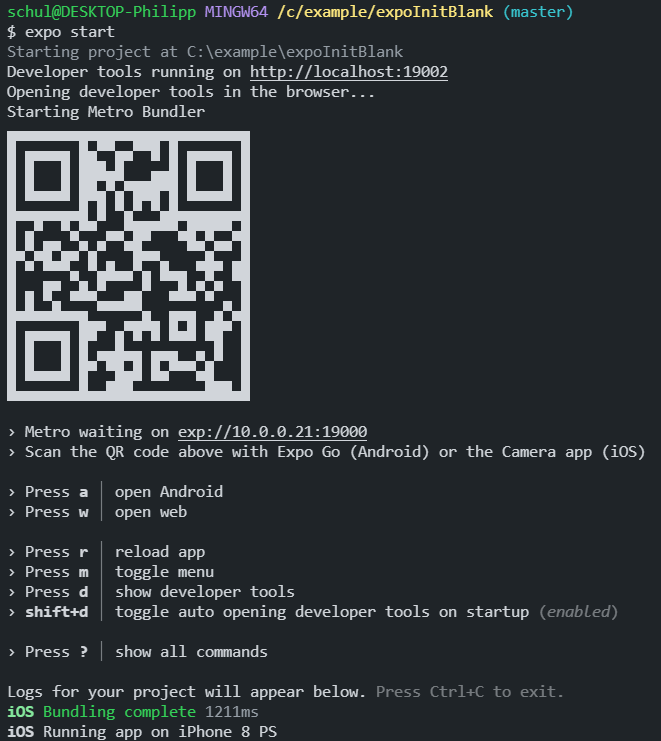
\includegraphics[width=0.6\textwidth]{Theorie/ReactNative/ExpoStart.png}
    \caption{Expo beim Start}
  \end{center}
\end{figure}

\begin{figure}[H]
  \begin{center}
    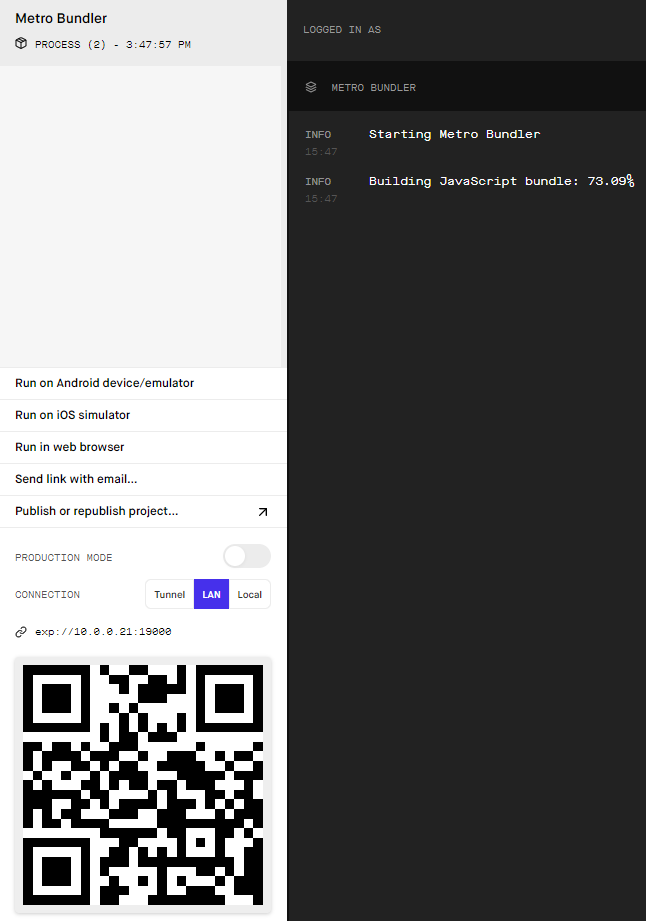
\includegraphics[width=0.6\textwidth]{Theorie/ReactNative/ExpoWebClient.png}
    \caption{Webinterface von Expo}
  \end{center}
\end{figure}

Nach dem Start wird im Webbrowser ein Entwickler-Menü geöffnet, auf dem noch einmal der QR-Code
und noch einige weitere hilfreiche Funktionen zu finden sind.

Um nun die App zu testen, muss man noch die ExpoGo App auf seinem Mobiltelefon installieren und den
gezeigten QR-Code scannen, während man im selben Netzwerk ist. Danach wird eine Bundle-Anfrage an
den lokalen Metro-Server geschickt, er kompiliert unser Projekt und schickt es an den Client.

\begin{figure}[H]
  \begin{center}
    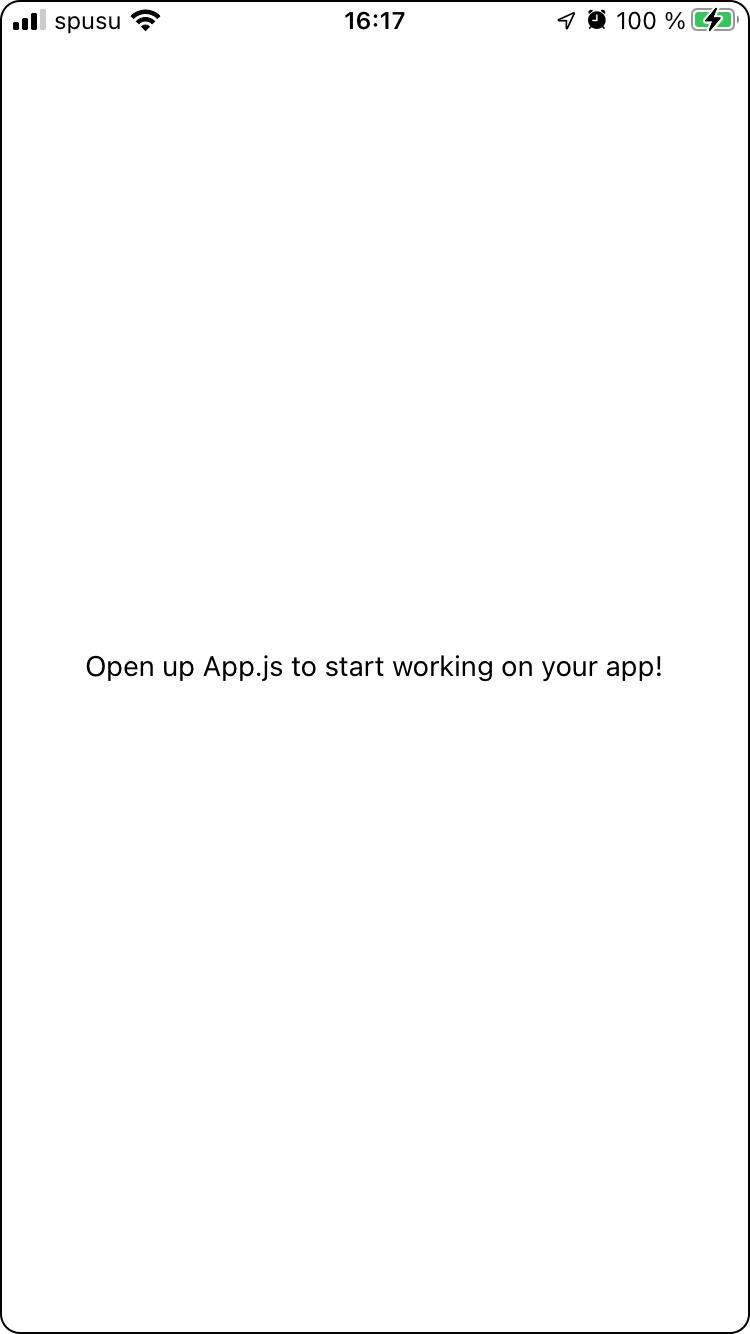
\includegraphics[width=0.5\textwidth]{Theorie/ReactNative/ExpoBlank.jpeg}
    \caption{Die weiße Leinwand von Expo}
  \end{center}
\end{figure}

\subsubsection{Expo Eject}
Wie bereits vorher schon erwähnt, hat es einige Nachteile seine App mit Expo zu machen. Um aber
einen schnellen Prototypen zu bauen ist das Framework perfekt. Um also eine Expo App in eine
vollwertige React Native Anwendung umzuwandeln, benötigt man folgenden Befehl.

\begin{lstlisting}
C:\example\expoInitBlank> expo eject
\end{lstlisting}

Man wird bei einer Eingabeaufforderung darüber informiert, dass dieser Prozess nicht rückgängig
gemacht werden kann. Danach sieht die Ordnerstruktur so aus:

\begin{figure}[H]
  \begin{center}
    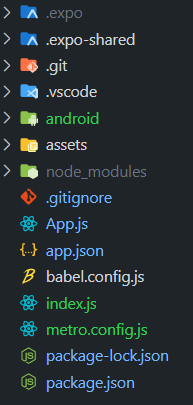
\includegraphics[height=0.5\textwidth]{Theorie/ReactNative/ExpoEject.png}
    \caption{Expo Eject Änderungen}
  \end{center}
\end{figure}

\begin{itemize}
  \item 
\end{itemize}

Um das Projekt für iOS-Geräte zu konfigurieren, führt man folgenden Befehl auf einem MacOS-PC aus:

\begin{lstlisting}
C:\example\expoInitBlank> npx pod-install
\end{lstlisting}



\subsubsection{React Native CLI}
Bei der Installationsanleitung auf der Webseite von React Native kann man sein aktuelles
Betriebssystem und Zielplattform auswählen. Apple erlaubt nicht die Entwicklung von Apps auf anderen
Betriebssystemen als MacOS selbst, d.h. die Entwicklung der App ist auf Windows 11, meinem
Betriebssystem, nicht möglich. Ich hatte auch während der Entwicklung nie Zugriff auf einen PC mit
MacOS, daher wurde die gesamte App ausschließlich für Android entwickelt. Doch sollten wir jemals
diese App wirklich veröffentlichen wollen, so wird das Umschreiben keinen großen Aufwand darstellen,
da wir immer darauf geachtet haben, nur Bibliotheken zu verwenden, die auch für iOS kompatibel sind.

\subsubsection{Abhängigkeiten und Erstellung des Projekts}
Für die Verwendung der React-Native-CLI werden einige andere Softwarepakete benötigt, darunter --
natürlich -- \nameref{nodejs}, mindestens Version 12. Außerdem wird benötigt:

\begin{itemize}
  \item Java SE Development Kit (mind. Version 11)
  \item Android Studio
  \begin{itemize}
    \item Android SDK 11 (R)
    \item Android SDK Platform: API Level 30
    \item Android Virtual Device: Google Pixel 2 mit Android 11
  \end{itemize}
\end{itemize}

Sobald alle Abhängigkeiten installiert wurden, führt man folgenden Befehl aus, um ein neues React
Native Projekt zu erstellen:

\begin{lstlisting}
C:\example> npx react-native init reactNativeInit
\end{lstlisting}

NPX ist ein Befehl, der seit Version 5.2.0 in NPM enthalten ist. Er ist speziell bei CLIs hilfreich,
denn anstatt das Paket react-native auf dem PC zu installieren und dann aufzurufen, wird mit dem
Befehl automatisch die neueste Version der CLI von einem Server abgefragt und ausgeführt. So kann
man sicherstellen, dass niemals eine veraltete Version der CLI verwendet wird.

Die App kann nun sofort getestet werden, als erstes startet man wieder den JavaScript-Bundler
\nameref{metrobundler} mit folgendem Befehl:

\begin{lstlisting}
C:\example\reactNativeInit> npm start
\end{lstlisting}

Dies ist die Kurzschreibweise für den Befehl npm run start. Start ist nämlich ein Skript in der
Datei package.json.

\begin{figure}[H]
  \begin{center}
    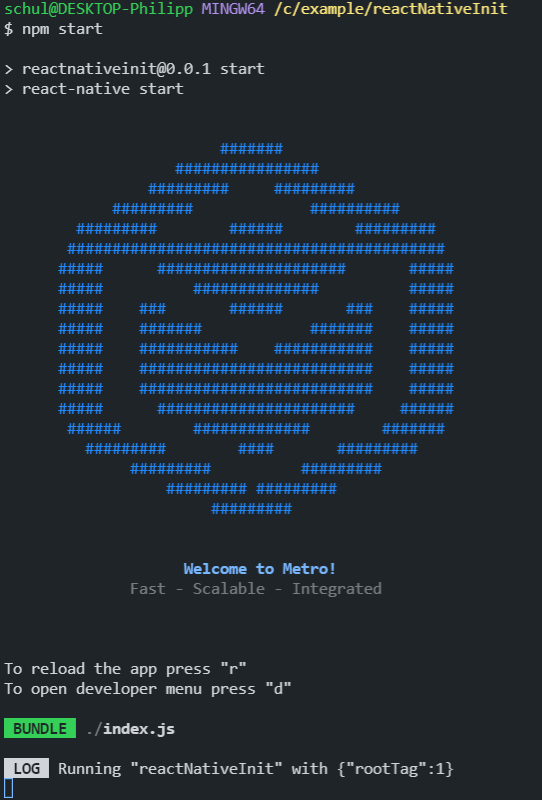
\includegraphics[width=0.5\textwidth]{Theorie/ReactNative/MetroBundler.png}
    \caption{Der Metro-Server in Aktion}
  \end{center}
\end{figure}

Als nächstes öffnet man den Ordner root/android in Android Studio. Man hat nun zwei Möglichkeiten,
die App auszuführen:

\begin{enumerate}
  \item Mit einem virtuellen Android Gerät (Android Virtual Device AVD):\\
Dazu öffnet man in Android Studio den AVD-Manager und erstellt einen neuen Emulator mit einer
Android Version von 11. Danach startet man den Emulator und führt folgenden Befehl aus:

\begin{lstlisting}
C:\example\reactNativeInit> npm run android
\end{lstlisting}

Die App wird auf dem Emulator installiert und ausgeführt.

\begin{figure}[H]
  \begin{center}
    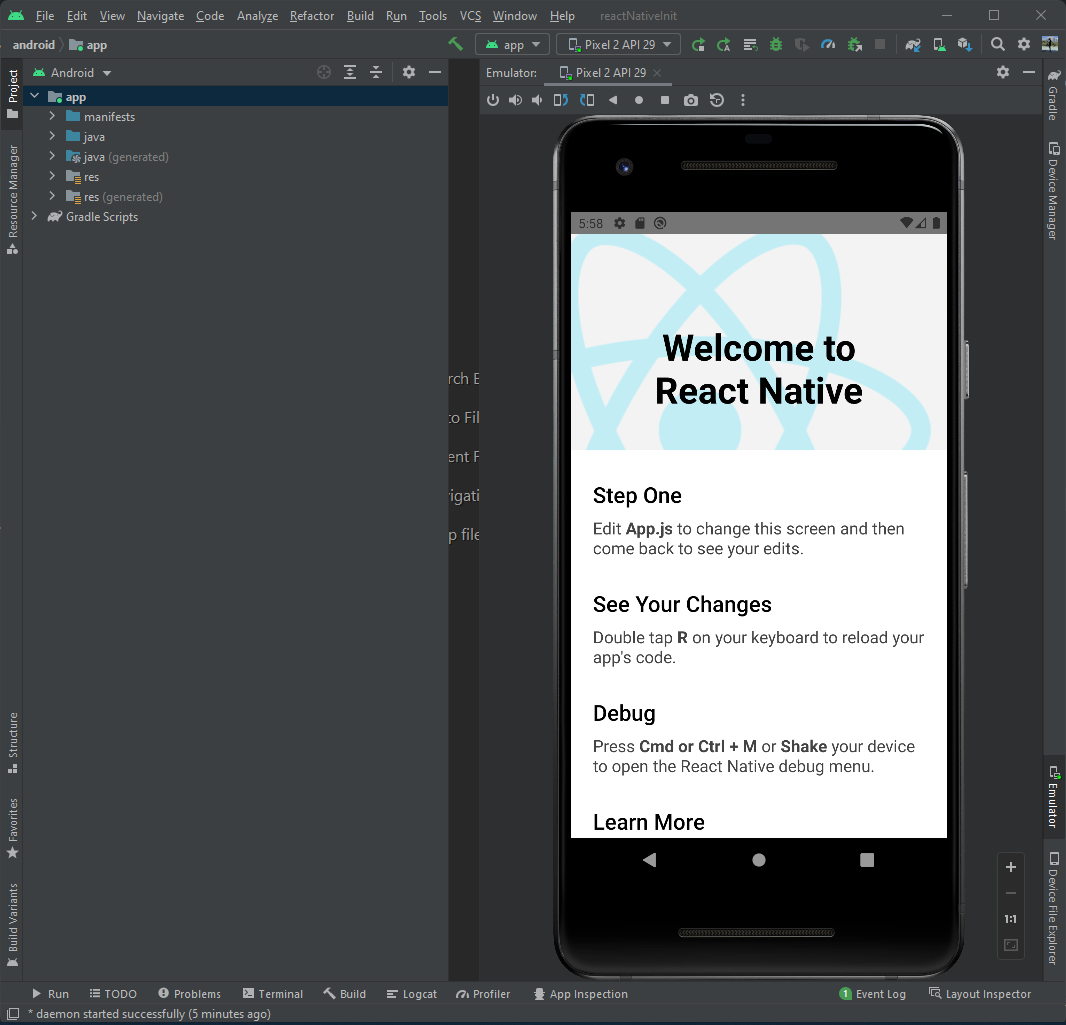
\includegraphics[width=0.8\textwidth]{Theorie/ReactNative/AndroidStudio.png}
    \caption{Die Beispiel-App in Android Studio}
  \end{center}
\end{figure}

  \item Mit einem physischen Android-Gerät:\\
Als erstes aktiviert man auf dem Gerät in den Einstellungen USB-Debugging und schließt es mittels
USB an den PC an. Wenn alle Treiber installiert sind, müsste es dann direkt in Android Studio
erkannt werden, um die App zu installieren.

Jetzt muss noch ein Tunnel über die USB-Verbindung erzeugt werden, damit das Gerät darüber mit dem
lokalen Metro-Server kommunizieren kann. Man listet alle Geräte auf und erzeugt dann mit der
Device-Identifikation einen Tunnel.

\begin{lstlisting}
C:\example\reactNativeInit> adb devices
List of devices attached
34299o5j85o496g3        device
emulator-8125           device

C:\example\reactNativeInit> adb -s 34299o5j85o496g3 reverse tcp:8081 tcp:8081
8081
\end{lstlisting}

\end{enumerate}

\subsubsection{Andere CLIs}
\begin{itemize}
  \item IgniteCLI \cite{ignitecli}
  \item Create-React-Native-App \cite{createReactNativeApp}
\end{itemize}
